\documentclass{beamer}

\usepackage{beamerthemesplit}
\usepackage{verbatim}
\usepackage[normalem]{ulem}

\usepackage{xcolor}

\usepackage{hyperref}

\definecolor{gold}{rgb}{1.,0.84,0.}
\definecolor{brightred}{rgb}{1.,0.4,0.4}
\definecolor{mygray}{RGB}{200,200,200}
\definecolor{lightsteelblue}{RGB}{176,196,222}
\definecolor{lightskyblue}{RGB}{135,206,250}
\definecolor{cadetblue}{RGB}{95,158,160}

\usetheme{default}
\usecolortheme{mule}

\usefonttheme{serif}

%\DeclareGraphicsExtensions{.pdf,.png,.jpg}

\newcommand{\mcal}{\textsc{metacalibration}}
\newcommand{\Mcal}{\textsc{Metacalibration}}

\newcommand{\mcalR}{\mbox{\boldmath $R$}}
\newcommand{\mcalRscalar}{\mbox{$R$}}

\newcommand{\mcalRmean}{\mbox{\boldmath $\langle R \rangle$}}
\newcommand{\mcalRscalarmean}{\mbox{$\langle R \rangle$}}

\newcommand{\mcalRpsf}{$R^{p}$}
\newcommand{\mcalRpsfnoise}{$R^{p}_\eta$}
\newcommand{\mcalRo}{\mbox{\boldmath $R_o$}}
\newcommand{\mcalRnoise}{\mbox{\boldmath $R_\eta$}}

\newcommand{\mcalRmeanalpha}{\mbox{\boldmath $\langle R_\alpha \rangle$}}
\newcommand{\mcalRmeanbeta}{\mbox{\boldmath $\langle R_\beta \rangle$}}

\newcommand{\mcalRg}{\mbox{\boldmath $R_\gamma$}}
\newcommand{\mcalRS}{\mbox{\boldmath $R_S$}}
\newcommand{\mcalRgmean}{\mbox{\boldmath $\langle R_\gamma \rangle$}}
\newcommand{\mcalRSmean}{\mbox{\boldmath $\langle R_S \rangle$}}

\newcommand{\mcalRtwopt}{\mbox{\boldmath $R^{2pt}$}}
\newcommand{\mcalRtwoptmean}{\mbox{\boldmath $\langle R^{2pt} \rangle$}}


\newcommand{\mcalRmodel}{\mbox{\boldmath $R^{model}$}}
\newcommand{\mcalRnoisemodel}{\mbox{\boldmath $R^{model}_\eta$}}


\newcommand{\vecg}{\mbox{\boldmath $\gamma$}}
\newcommand{\vest}{\mbox{\boldmath $e$}}

\newcommand{\snr}{$S/N$}
\newcommand{\snT}{$(S/N)_{\textrm{size}}$}
%\newcommand{\snT}{$\left( \frac{S}{N}\right)_{\textrm{size}}$}
\newcommand{\snflux}{$(S/N)_{\textrm{flux}}$}
%\newcommand{\snflux}{$\left( \frac{S}{N}\right)_{\textrm{flux}}$}

\newcommand{\lensfit}{\texttt{LENSFIT}}
\newcommand{\numba}{\texttt{Numba}}
\newcommand{\python}{\texttt{Python}}
\newcommand{\ngmix}{\texttt{ngmix}}
\newcommand{\shear}{{\bf g}}
\newcommand{\redmapper}{redMaPPer}
\newcommand{\est}{$e$}


\newcommand{\prelim}{{\bf{\it Preliminary}}}

\newcommand{\uberseg}{{\"u}berseg}


\title{Effect of Neighbors on \mcal\ Shear Estimation}
\author{Erin Sheldon}
\institute{Brookhaven National Laboratory}

% http://texblog.net/latex-archive/plaintex/beamer-footline-frame-number/
% to add the page (frame ) number and not screw up the bottom line
% works for split themes?
\expandafter\def\expandafter\insertshorttitle\expandafter{%
      \insertshorttitle\hfill%
        \insertframenumber\,/\,\inserttotalframenumber}

% suppress navigation bar
\beamertemplatenavigationsymbolsempty
\setbeamertemplate{footline}{}

\begin{document}

\usebackgroundtemplate{%
    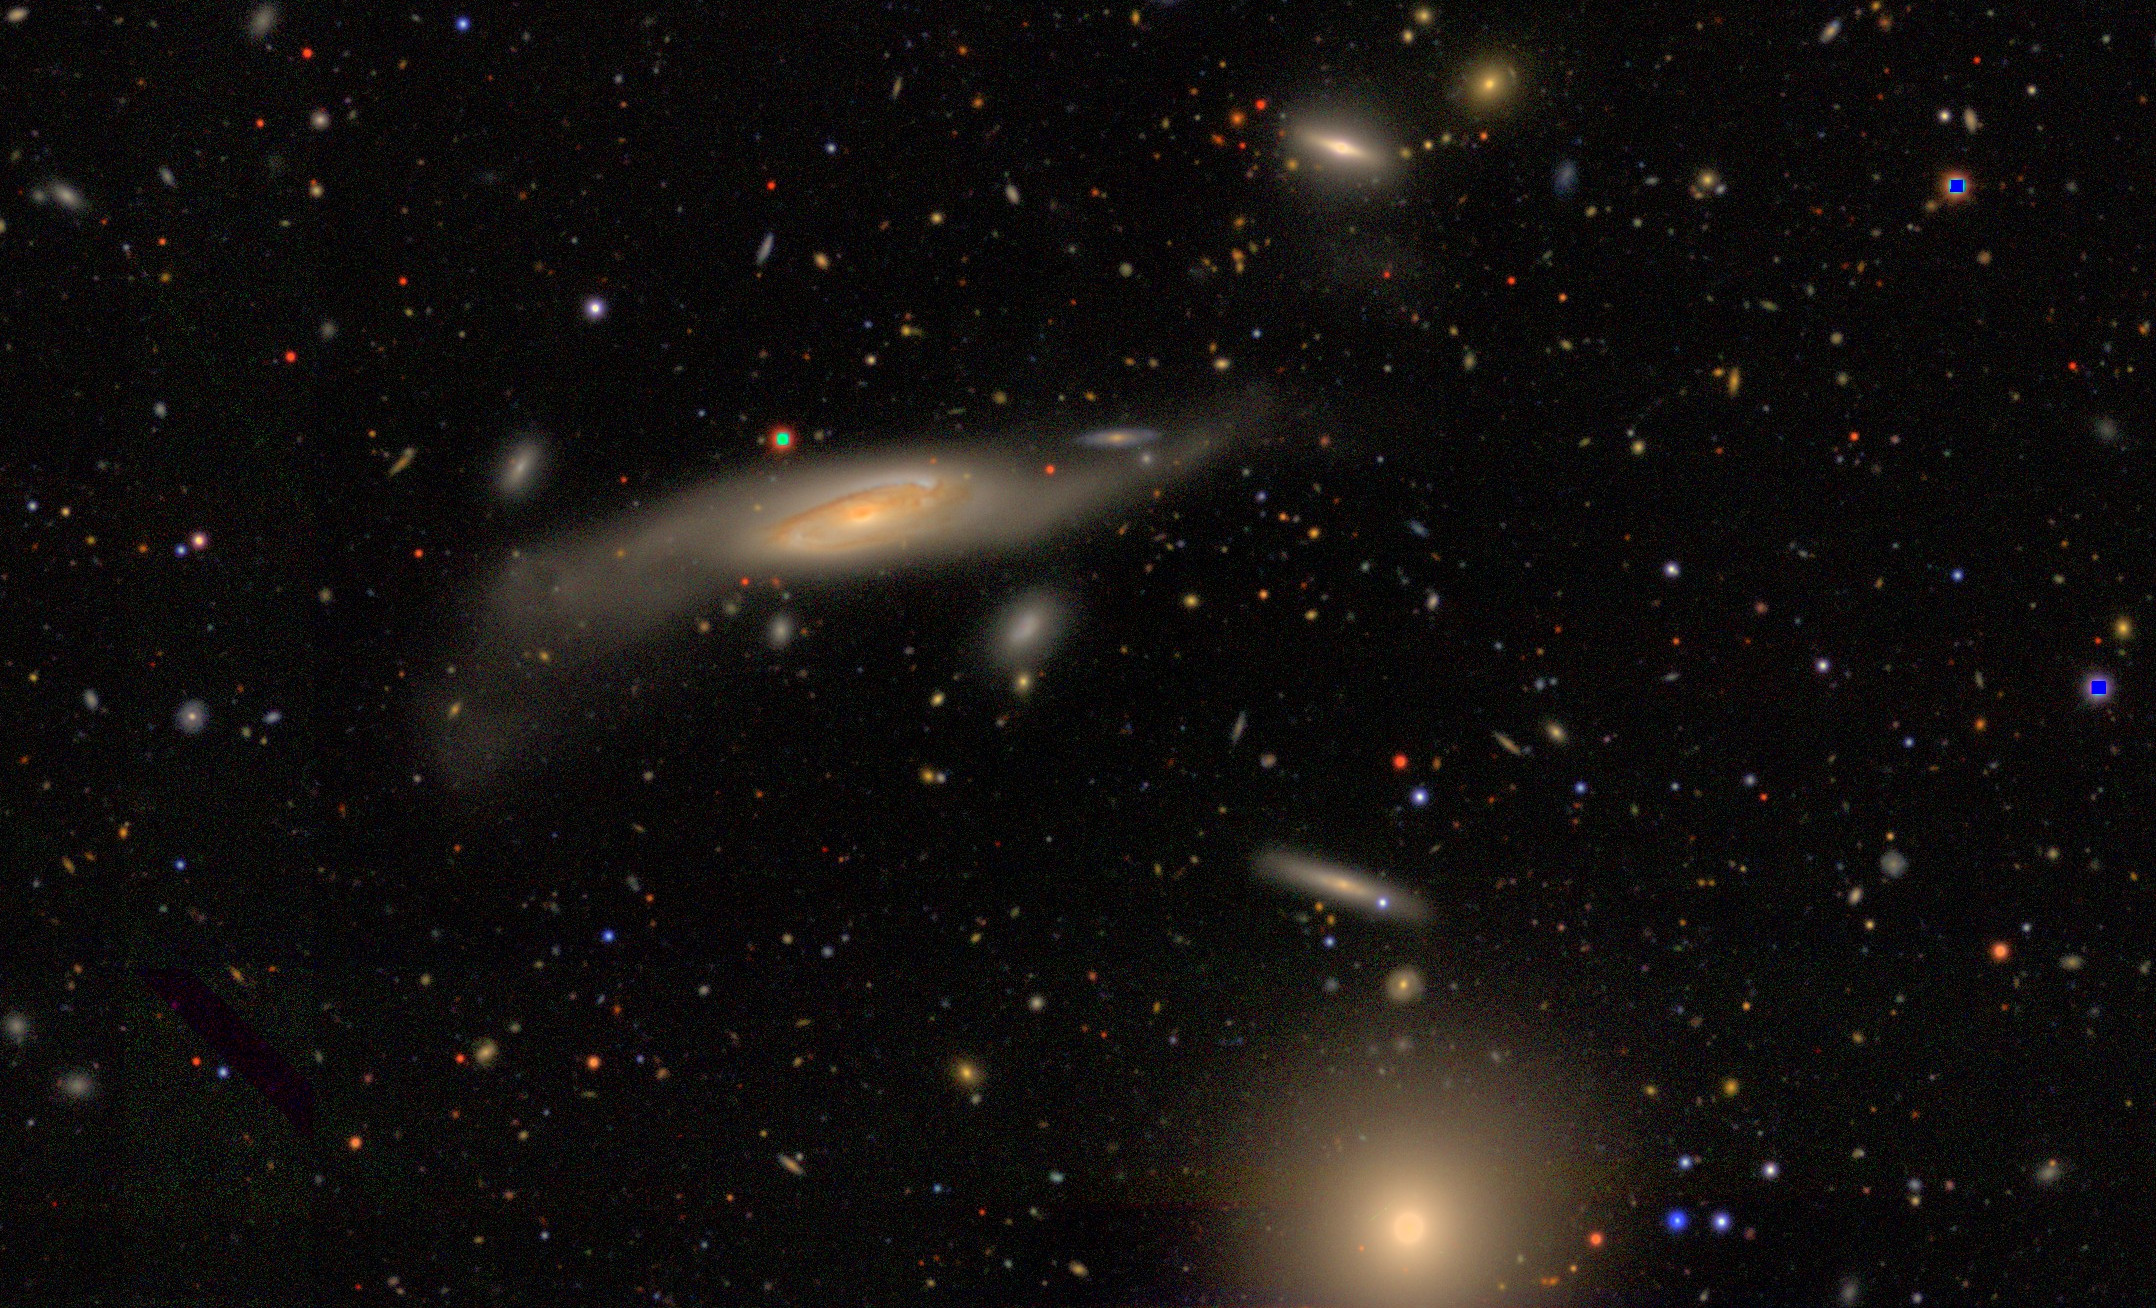
\includegraphics[height=\paperheight]{DES0056-5248_gri_crop.jpg}}
\frame
{
}
\setbeamertemplate{background canvas}[vertical shading][bottom=mgray,top=mblack]

\setbeamerfont*{itemize/enumerate body}{size=\Large}
\setbeamerfont*{itemize/enumerate subbody}{parent=itemize/enumerate body}
\setbeamerfont*{itemize/enumerate subsubbody}{parent=itemize/enumerate body}


\frame{\titlepage}




\frame
{
    \frametitle{Outline}

    \begin{itemize}

        \item Simulations
        \item Performance with and without MOF neighbor subtraction
        \item Future Work

    \end{itemize}

}

\frame
{
    \frametitle{Too Close for Comfort}
 
    \setbeamerfont*{itemize/enumerate body}{size=\normalsize}
    \setbeamerfont*{itemize/enumerate subbody}{parent=itemize/enumerate body}
    \setbeamerfont*{itemize/enumerate subsubbody}{parent=itemize/enumerate body}
 
    \begin{columns}
        \begin{column}{0.5\textwidth}
            \begin{itemize}
                \item \mcal\ will calculate the correct response
                    for blended objects.
                \item Good enough if they are at the same redshift
                \item If they are at different redshifts, then must
                    identify unique objects and separately
                    determine their redshifts and \mcal\ responses.
            \end{itemize}
        \end{column}
        \begin{column}{0.5\textwidth}
            \begin{center}
                %\includegraphics[width=\textwidth]{DES0428-4748_gri_crop.jpg}
                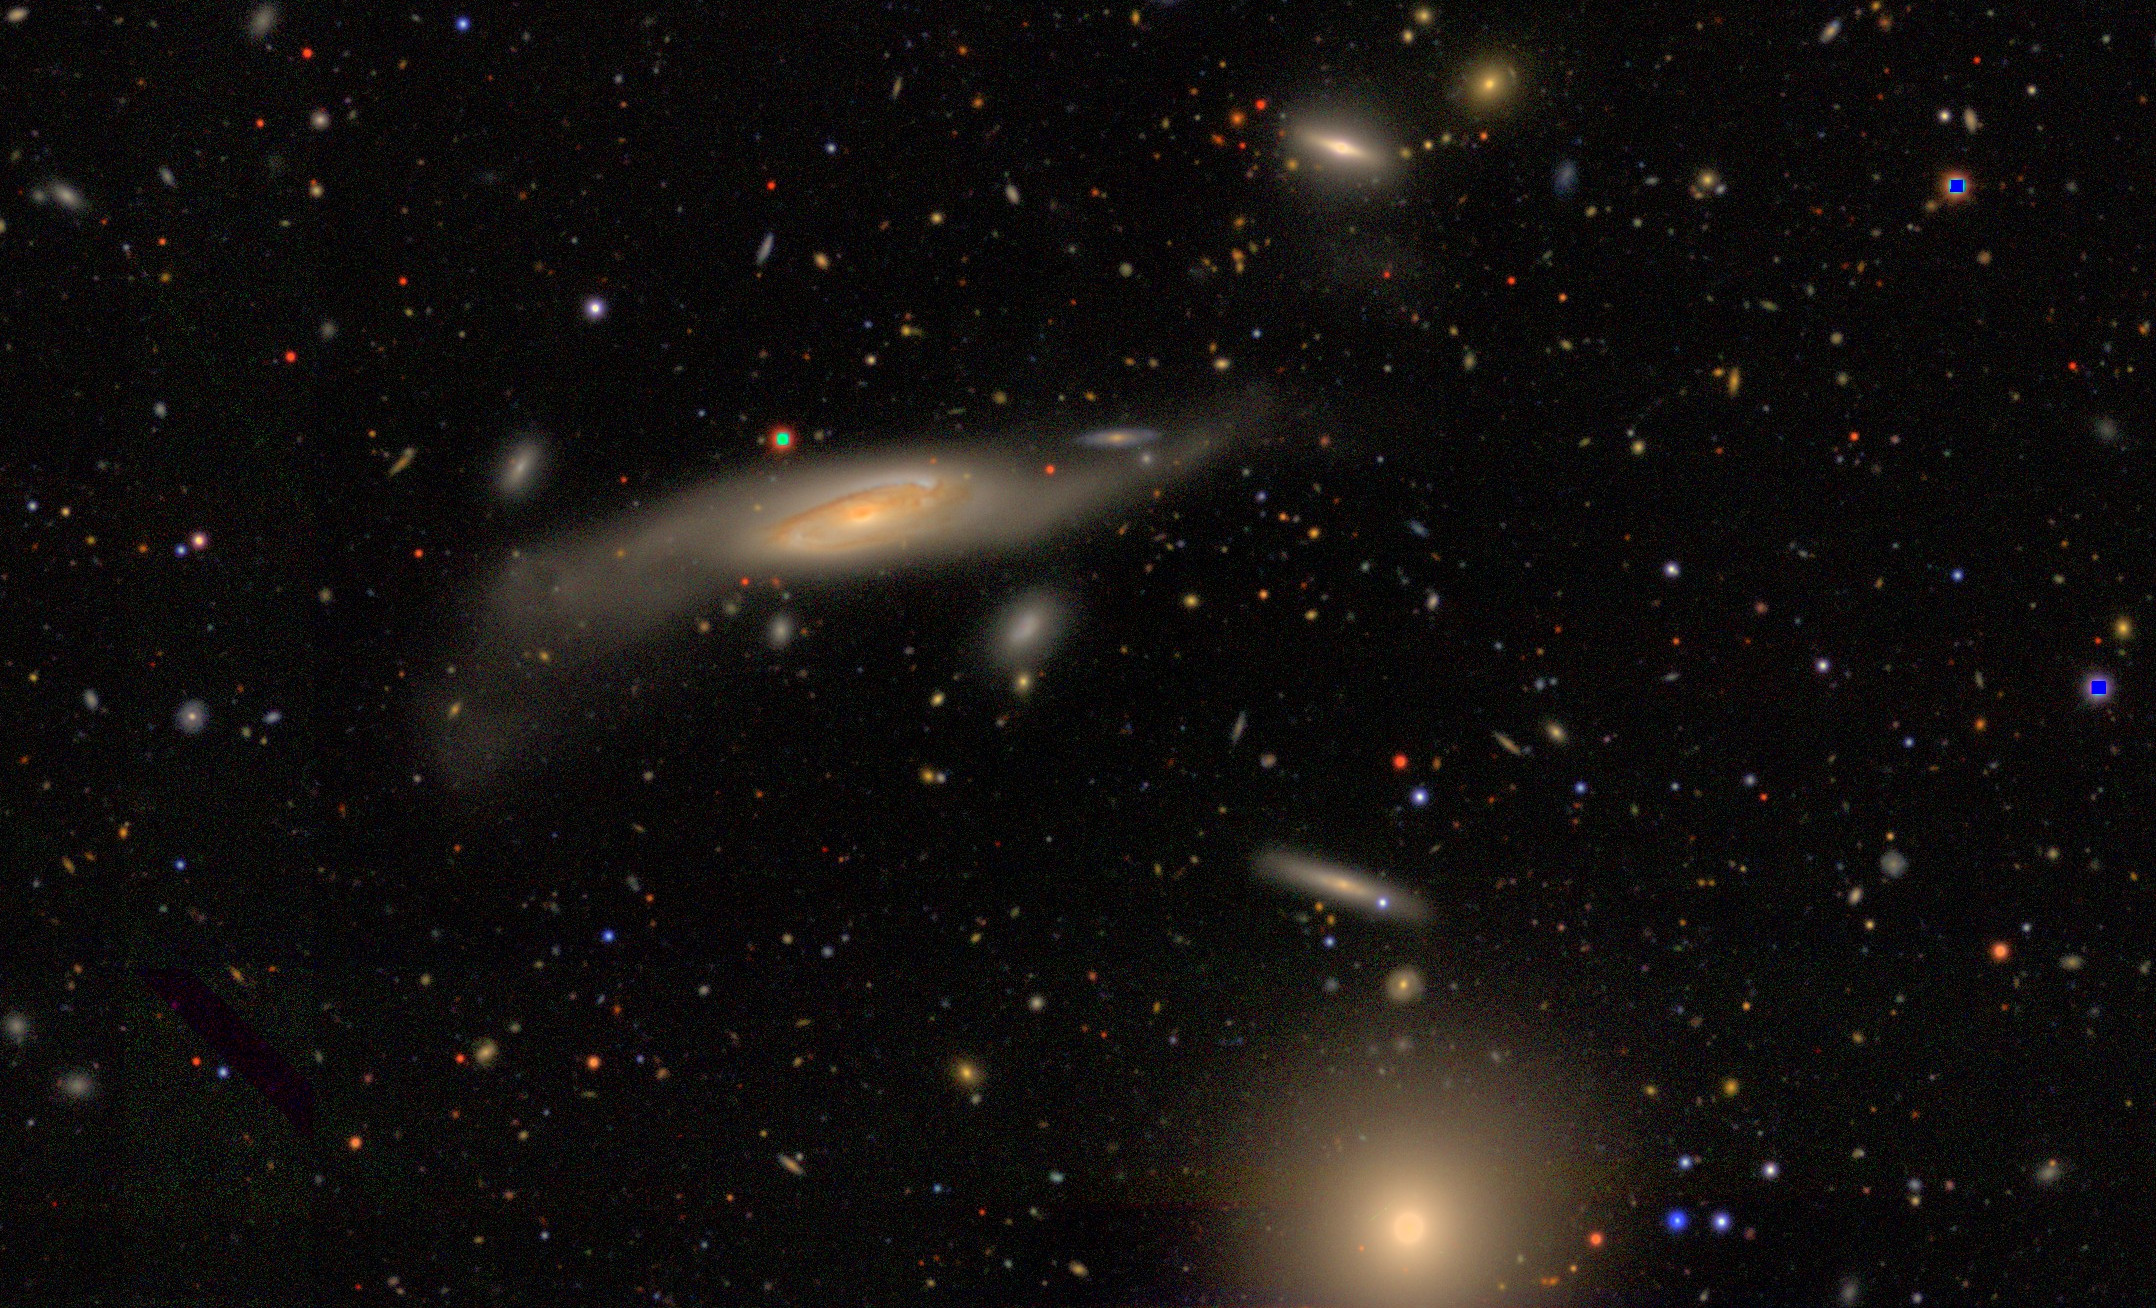
\includegraphics[width=1.2\textwidth, angle=90]{DES0056-5248_gri_crop.jpg}
            \end{center}
        \end{column}
    \end{columns}


}




\frame
{

    \frametitle{Simulation}

    \setbeamerfont*{itemize/enumerate body}{size=\large}
    \setbeamerfont*{itemize/enumerate subbody}{parent=itemize/enumerate body}
    \setbeamerfont*{itemize/enumerate subsubbody}{parent=itemize/enumerate body}

    \begin{itemize}
        \item Galsim
        \item Flux/size drawn jointly from COSMOS 25.2 sample

        \item ``Fake'' a fainter sample to mag 27.5 by scaling
            the flux and size of 25.2 sample.  Also fake extra bright galaxies.

        \item Bulge+Disk with different ellipticities/orientation.
        \item Knots of star formation (\texttt{galsim.RandomWalk})

        \item Half galaxies get shear 0.01, half get 0.02

        \item Place galaxies randomly on images mimicking DES coadds

        \item Add noise to achieve DES 5-year depth in $i\approx 24.1$

        \item Run through SExtractor, make MEDS files.

        \item PSF Moffat $e=0.05$, FWHM = 0.9 arcsec.
    \end{itemize}

}

{

    %\setbeamertemplate{background canvas}[vertical shading][bottom=white,top=white]
    \frame
    {
        \frametitle{Example Galaxies}
     
        {\small Large examples to show internal structure:  actual simulation
        galaxies are almost all smaller than the PSF }

        \begin{center}
            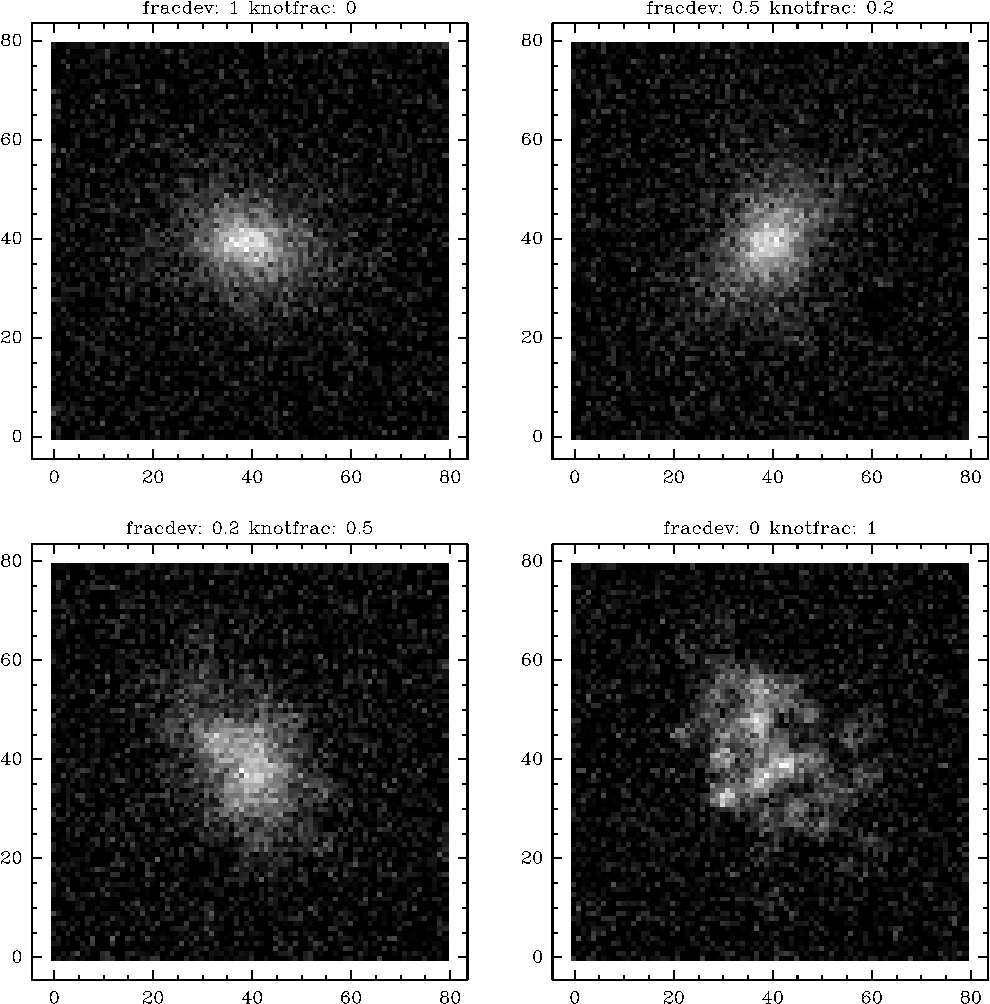
\includegraphics[width=0.7\textwidth]{mosaic-009086.pdf}
            \newline
        \end{center}

    }
    %\setbeamertemplate{background canvas}[vertical shading][bottom=mgray,top=mblack]


}



\frame
{
    \frametitle{Simulation for Deblending Tests }
 
    \begin{center}
        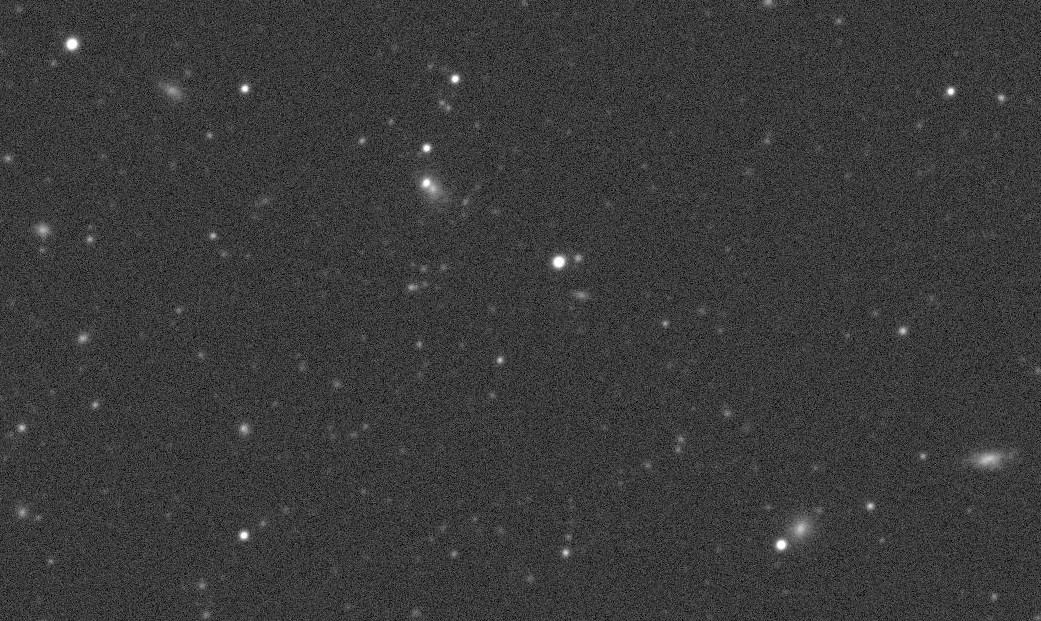
\includegraphics[width=\columnwidth]{nbrsim-003f-009969-image-crop.jpg}
    \end{center}

}


\frame
{

    \frametitle{Results for Deblending Tests}

    \setbeamerfont*{itemize/enumerate body}{size=\large}
    \setbeamerfont*{itemize/enumerate subbody}{parent=itemize/enumerate body}
    \setbeamerfont*{itemize/enumerate subsubbody}{parent=itemize/enumerate body}


    \begin{itemize}

        \item Run in two modes
        \item Mask neighbors using \uberseg\ algorithm (Jarvis et al. 2016)
            \begin{itemize}
                \item Use pixels closer to this object than any other.
                \item Don't use pixels assigned to another
                    object in the SExtractor segmentation map
            \end{itemize}

        \item Subtract the light from neighbors using the multi-object
            fitting (MOF: Matt Becker, Erin Sheldon)
            \begin{itemize}
                \item Fit blended objects semi-simultaneously (I can give details)
                \item https://github.com/esheldon/ngmix
                \item https://github.com/esheldon/ngmixer
            \end{itemize}

        \item \uberseg-only is the catalog we are using in Y1, because we
            lack photozs for the \uberseg+MOF catalog.

    \end{itemize}


}

\frame
{

    \frametitle{Results for Deblending Tests}

    \begin{table}
        \centering
        \begin{tabular}{ l c c}
            \hline
            Method         & \snr\ Cut & m            \\
                       &           & $[10^{-2}]$  \\
            \hline
            \hline

            \uberseg       & \snr$ > 10$ & 2.18 $\pm$ 0.16  \\
            \uberseg       & \snr$ > 15$ & 1.73 $\pm$ 0.17  \\
            \uberseg       & \snr$ > 20$ & 1.74 $\pm$ 0.18  \\


            \hline

            \uberseg+MOF   & \snr$ > 10$ & 0.10 $\pm$ 0.20  \\
            \uberseg+MOF   & \snr$ > 15$ & -0.24 $\pm$ 0.21 \\
            \uberseg+MOF   & \snr$ > 20$ & -0.04 $\pm$ 0.22 \\



            \hline
        \end{tabular}

        \caption{\snr\ cuts in addition to flags$<= 3$ and
        $T/T_{\mathrm{PSF}} > 0.5$}
    \end{table}


}

\frame
{

    \frametitle{Comparison with Test on DES Data}

    \begin{itemize}

        \item $\approx$2\% bias for \uberseg-only, no bias
            for MOF+\uberseg

        \item Would not take the 2\% number as indicative of the actual $m$ in
            DES, the simulations do not match real data perfectly.
            \begin{itemize}

                \item Galaxies have the right size-flux distribution,
                    approaching the complexity of real galaxies, but detailed
                    properties not tuned to real data

                \item Density is Y5 depth, greater than Y1

            \end{itemize}

    \end{itemize}
}
\frame
{

    \frametitle{Comparison with Test on DES Data}


    \begin{itemize}

        \item Test by Daniel Gruen in DES data

        \item \uberseg+MOF also $\approx$2.4\% lower than \uberseg\ alone.

        \item When limiting to objects with few neighbors, we find $0.011 \pm 0.013$,
            no longer detected, which is expected.

        \item 2\% agrees remarkably well with the simulation value, but note the
            simulation is higher density than Y1 so we would expect the effect
            to be lower in Y1.

        \item Could be \uberseg\ is biased, or both are biased differently.  Adopting
            a prior of $m = 0.012 \pm 0.012$ which overlaps zero and 2.4\% at $1-\sigma$.


    \end{itemize}


}





\frame
{
    \frametitle{Future Work}

    \begin{itemize}

        \item Do we trust that \uberseg+MOF is unbiased in real data?

        \item Try to break it

        \item Evolve these simulations toward full validation, adding
            additional realism, but retaining the ability to turn on and off
            various effects.

        \item Insert galaxy clusters into sim

        \item Put in realistic galaxy clustering

    \end{itemize}
}




\end{document}
